\begin{frame}
\frametitle{Эксперимент: Взаимная Информация (MI)}

\onslide<1->{\begin{figure}
    \centering
    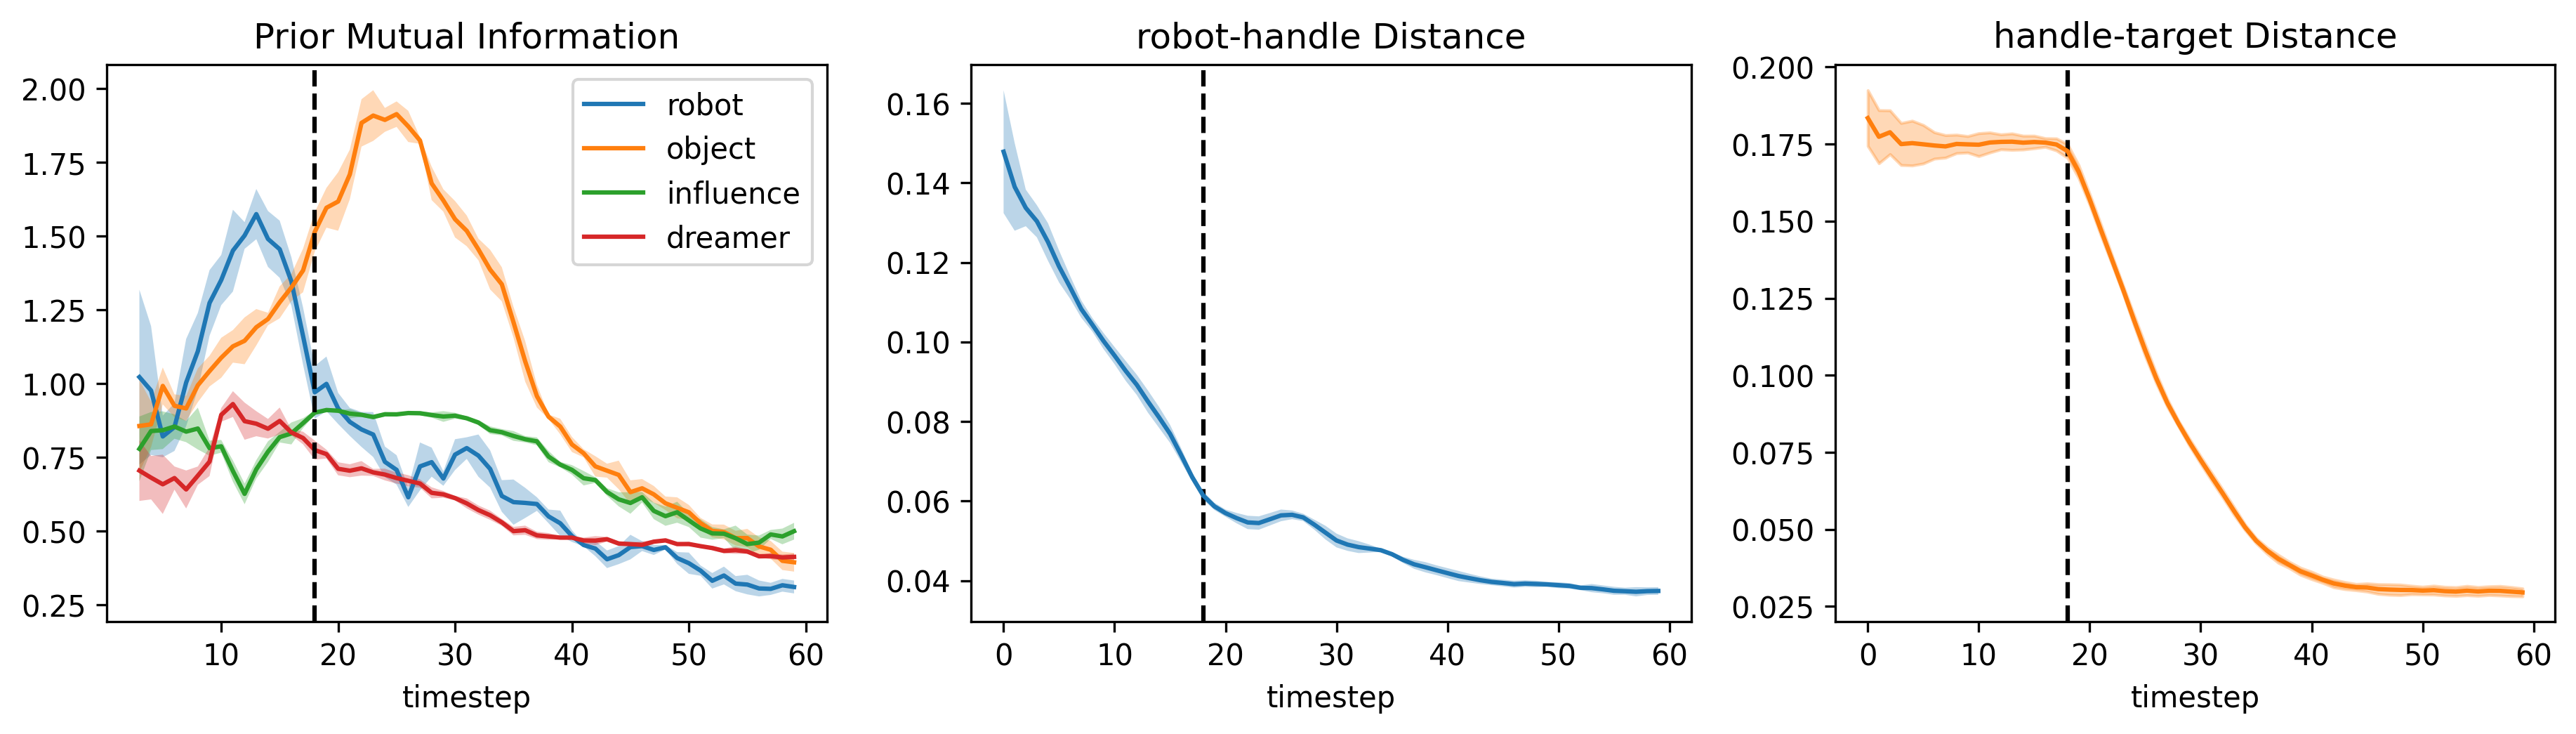
\includegraphics[width=0.95\linewidth]{images/mi_plots/mi_plot.png}
    \caption{Взаимная информацию между входом и выходом различных частей модели мира агента.}
\end{figure}
}
\note[item]<1->{To show how the model can reflect the cause-effect relationships, we study the excitement measure for each conditional distribution, i.e. Conditional Mutual Information between input and output of state distributions. Results show that distributions are activated in bottom-up fashion from robot to object part, propagating influence of actions on object.}
\onslide<2->{\begin{figure}[t]
    \centering
    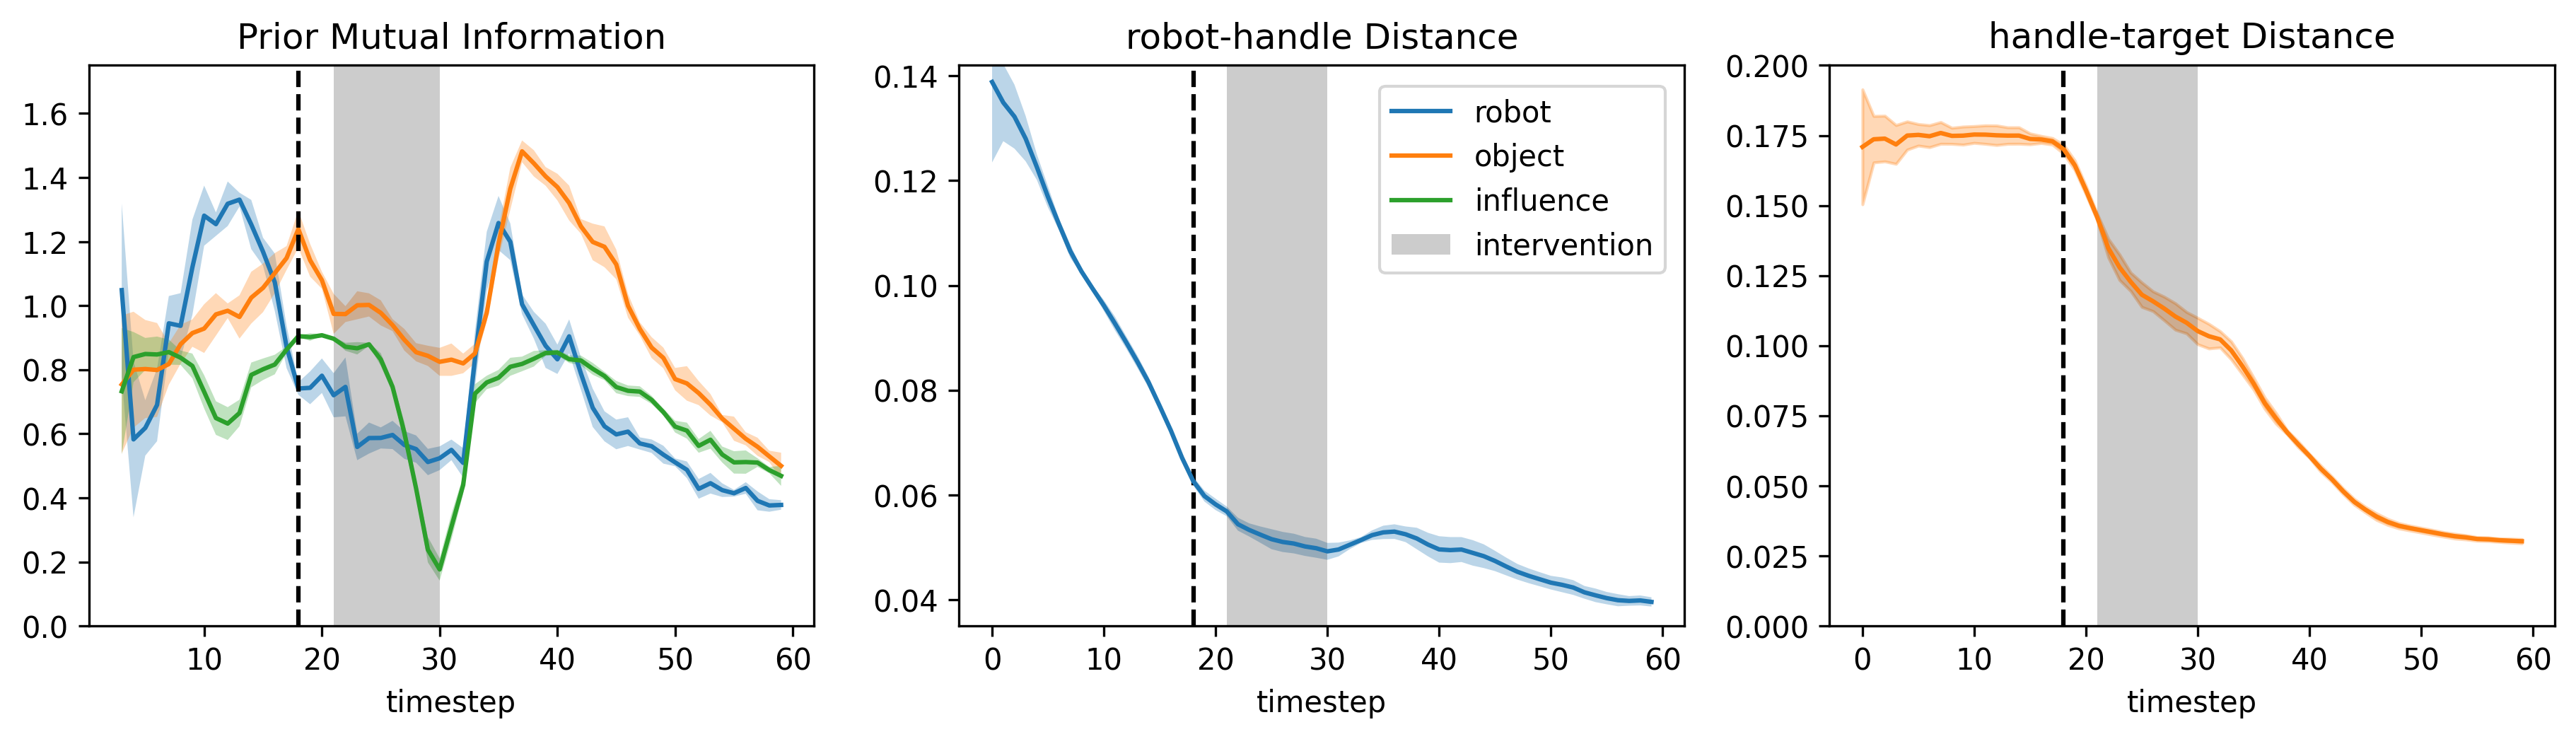
\includegraphics[width=0.95\linewidth]{images/mi_plots/mi_plot_interventions.png}
    \caption{Взаимная информация в условиях искусственного вмешательства в эпизод\footnotemark.}
\end{figure}
}
\onslide<2->{\scriptsize{* В середине открытия ящика, движение всех объектов в среде заморожено путем искусственной вставки нескольких пустых действий.}
}
\note[item]<2->{Also, we conducted the experiment involving stopping the robot hand while it has just begun closing the box. Just after resuming, robot continues to affect the drawer, which results in even faster response in influence state, which, in turn, affects the object state.}
\end{frame}